%%%%%%%%%%%%%%%%%%%%%%%%%%%%%%%%%%%%%%%%%%%%%%%%%%%%%%%%%%%%%%%%%%%%%%%%
%
% Template latex file for a common article class for class notes
% and write ups. Additional Configuration and styling options are 
% commented out. ex. Table of Contents and Title page
% 
% Author: Amy Bui
%
%%%%%%%%%%%%%%%%%%%%%%%%%%%%%%%%%%%%%%%%%%%%%%%%%%%%%%%%%%%%%%%%%%%%%%%%

\documentclass[12pt]{article}
\usepackage[utf8]{inputenc}
\usepackage{parskip}
\usepackage{tabularx}
\usepackage{caption}
\usepackage{subcaption}
\usepackage[color, leftbars]{changebar}

% Important Configurations

%%%%%%%%%%%%%%%%%%%%%%%%%%%%%%%%%%%%%%%%%%%%%%%%%%%%%%%%%%%%%%%%%%%%%%%%
% Reduce margin
%
% \addtolength{\oddsidemargin}{-.85in}
% \addtolength{\evensidemargin}{-.85in}
% \addtolength{\textwidth}{1in}

% \addtolength{\topmargin}{-.85in}
% \addtolength{\textheight}{1in}

% Page format commands:
% Override normal article margins,
% making the margins smaller
\setlength{\textwidth}{6.5in}
\setlength{\textheight}{9in}
\setlength{\oddsidemargin}{0in}
\setlength{\evensidemargin}{0in}
\setlength{\topmargin}{-0.5in}

\setlength{\parindent}{0pt}
%%%%%%%%%%%%%%%%%%%%%%%%%%%%%%%%%%%%%%%%%%%%%%%%%%%%%%%%%%%%%%%%%%%%%%%%


%%%%%%%%%%%%%%%%%%%%%%%%%%%%%%%%%%%%%%%%%%%%%%%%%%%%%%%%%%%%%%%%%%%%%%%%
% Math Symbols
\usepackage{mathtools}
\usepackage{amssymb}
% \usepackage{epsfig}
\usepackage{amsmath,amsthm}
\usepackage{amscd,amsxtra,latexsym}


% add floor and ceiling symbol. Usage: \ceil*{}, \floor*{}
\DeclarePairedDelimiter\ceil{\lceil}{\rceil}
\DeclarePairedDelimiter\floor{\lfloor}{\rfloor}

% multiset \langle ... \rangle
\def\multiset#1#2{\ensuremath{\left(\kern-.3em\left(\genfrac{}{}{0pt}{}{#1}{#2}\right)\kern-.3em\right)}}



%%%%%%%%%%%%%%%%%%%%%%%%%%%%%%%%%%%%%%%%%%%%%%%%%%%%%%%%%%%%%%%%%%%%%%%%

%%%%%%%%%%%%%%%%%%%%%%%%%%%%%%%%%%%%%%%%%%%%%%%%%%%%%%%%%%%%%%%%%%%%%%%%
% Code Sample Styling

% use \lstinline! xxx ! or \begin{lstlisting} ... \end{lstlisting}
\usepackage{listings}

\usepackage{color}
\definecolor{light-gray}{gray}{0.97} % shade of grey
\definecolor{dkgreen}{rgb}{0,0.6,0}
\definecolor{gray}{rgb}{0.5,0.5,0.5}
\definecolor{mauve}{rgb}{0.58,0,0.82}

% \begin{lstlisting}[...] ... \end{lstlisting}
\lstset{frame=none,
    language=C++,
    aboveskip=3mm,
    belowskip=3mm,
    stepnumber=1, % set to 0 if you don't like line nums
    showstringspaces=false,
    columns=flexible,
    basicstyle={\small\ttfamily},
    numbers=left,
    numberstyle=\color{black},
    keywordstyle=\color{blue},
    commentstyle=\color{dkgreen},
    stringstyle=\color{mauve},
    backgroundcolor=\color{light-gray},
    breaklines=true,
    breakatwhitespace=false,
    tabsize=2
}



%%%%%%%%%%%%%%%%%%%%%%%%%%%%%%%%%%%%%%%%%%%%%%%%%%%%%%%%%%%%%%%%%%%%%%%%

%%%%%%%%%%%%%%%%%%%%%%%%%%%%%%%%%%%%%%%%%%%%%%%%%%%%%%%%%%%%%%%%%%%%%%%%
\usepackage{xcolor}
%% https://tex.stackexchange.com/questions/401750/quick-and-short-command-for-coloring-one-word
\newcommand\shorthandon{\catcode`@=\active \catcode`^=\active \catcode`*=\active }
\newcommand\shorthandoff{\catcode`@=12 \catcode`^=7 \catcode`*=12 }
\shorthandon
\def@#1@{\textcolor{red}{#1}}%
\def^#1^{\textcolor{blue}{#1}}%
\def*#1{\string#1}
\shorthandoff
%% useage: \textcolor{red}{text here}
% \shorthandon
% This is a @test@ of the ^emergency^ bro*@dcast system.
% \shorthandoff
%%%%%%%%%%%%%%%%%%%%%%%%%%%%%%%%%%%%%%%%%%%%%%%%%%%%%%%%%%%%%%%%%%%%%%%%


%%%%%%%%%%%%%%%%%%%%%%%%%%%%%%%%%%%%%%%%%%%%%%%%%%%%%%%%%%%%%%%%%%%%%%%%

%Commands below change page margins (this much space at the titlepage, etc)
\newlength{\toppush}
\setlength{\toppush}{2\headheight}
\addtolength{\toppush}{\headsep}

% Section header Styling
% The commands below change the bold text where it says "Section" into "Question"
% \usepackage{titlesec}
% \titleformat{\section}
% {\normalfont\Large\bfseries}{Question~\thesection:}{1em}{}

% I added this command below to chance "subsections numbers" to be "Question [subsection number]" -AB 1/31/2021
% \titleformat{\subsection}
% {\normalfont\bfseries}{\thesubsection:}{1em}{}

% Page head Styling
% Name and subject of the class
\def\subjnum{Comp 163}          % Class Number
\def\subjname{CompGeo}       % Class Name

% Name of the student, university name and which semester
\def\doheading#1#2#3{\vfill\eject\vspace*{-\toppush}%
  \vbox{\hbox to\textwidth{{\bf} \subjnum: \subjname \hfil Amy Bui}%
    \hbox to\textwidth{{\bf} Tufts University, Fall 2022 \hfil#3\strut}%
    \hrule}}

%Command for the title of the document (Homework 0)
\newcommand{\htitle}[1]{\vspace*{1.25ex plus 1ex minus 0ex}%
\begin{center}
    {\large\bf #1}
\end{center}} 
%%%%%%%%%%%%%%%%%%%%%%%%%%%%%%%%%%%%%%%%%%%%%%%%%%%%%%%%%%%%%%%%%%%%%%%%



%%%%%%%%%%%%%%%%%%%%%%%%%%%%%%%%%%%%%%%%%%%%%%%%%%%%%%%%%%%%%%%%%%%%%%%%
% Misc
\usepackage{graphicx} % graphics
\usepackage{enumitem} % listing style (bullet lists)

% below helps with trying to get figures in a row
% \usepackage{caption}
% \usepackage{subcaption}

% hyperlink styling
% use \href{} and \url{}, and colors table of contents links
% use \href{} and \url{}
% \label{sec:name}
% \hyperref[label]{text}
\usepackage{hyperref}
\hypersetup{
    colorlinks=true,
    linkcolor=blue, % was previously black
    filecolor=magenta,
    urlcolor=blue,
    pdftitle={Template}
}
\urlstyle{same}

% A command for primes (')
\newcommand{\p}%
    {\ensuremath{^{\prime}}}

% a command for double primes ('')
\newcommand{\pp}%
    {\ensuremath{^{\prime \prime}}}

% A command for the Kleene star
\newcommand{\str}%
    {\ensuremath{^{\star}}}

% a command for the double star
\newcommand{\sstr}%
    {\ensuremath{^{\star\star}}}
%%%%%%%%%%%%%%%%%%%%%%%%%%%%%%%%%%%%%%%%%%%%%%%%%%%%%%%%%%%%%%%%%%%%%%%%

% Options for title page, use \maketitle in document
% \author{Amy Bui}
% \title{COMP160 - Algorithms: Class Notes and Practice}

\begin{document}
%% create title page
% \title{(g)ROOT \\ Language Reference Manual}
% \author{Samuel Russo \quad Amy Bui \quad Eliza Encherman \\ Zachary Goldstein \quad Nickolas Gravel}
% \date{\today}
% \maketitle

\doheading{2}{title}{Notes}

    %%%%%%%%%%%%%%%%%%%%%%%%%%%%%%%%%%%%%%%%%%%%%%%%%%%%%%%%%%%%%%%%%%%%%%%%
    % Table of Contents
    \setcounter{tocdepth}{2}
    \tableofcontents
    \pagebreak
    %%%%%%%%%%%%%%%%%%%%%%%%%%%%%%%%%%%%%%%%%%%%%%%%%%%%%%%%%%%%%%%%%%%%%%%%

    %%%%%%%%%%%%%%%%%%%%%%%%%%%%%%%%%%%%%%%%%%%%%%%%%%%%%%%%%%%%%%%%%%%%%%%%
    \section{Intro: Computational Geometry - A User's Guide (Notes)}
    \label{sec:compgeointro}
    Introduction to algorithims for computations that are geometric in nature. Souvaine \& Dobkin describe some methods with geometric applications.

    Three families of Geometric Algorithms:
    \begin{itemize}
        \item Decomposition of problem into subproblems -- \hyperref[subsec:hsm]{Hierarchical Searching Method} 
        \item Decomposition of problem into subproblems -- \hyperref[subsec:dcm]{Divide and Conquer Method}
        \item Transform a problem into a new (maybe more tractable) format -- \hyperref[subsec:dualitym]{Duality Method}
    \end{itemize}

    Geometric Principles
    \begin{itemize}
        \item Planar Point Location
        \item Convex Hull Construction and Updating
        \item Computation of Polygon
        \item Computation of Disk
        \item Computation of Half-Space Intersections
    \end{itemize}

        %%%
        \subsection{Hierarchical Searching Method}
        \label{subsec:hsm}
            \begin{itemize}
                \item Geometric problem is preprocessed to a coarse representation, such that it can be broken down, and search queries can be called on localized region where the problem is solved. 
                \item Algorithmic efficiency is then balanced against preprocessing time and storage space requirements. 
                \item Binary Search of Sorted Array 
            \end{itemize}

            \subsubsection{\href{https://www.geeksforgeeks.org/binary-search/}{Binary Search} on Geometric Problems}
                \begin{description}
                    \item[Input:] A collection of $N$ disjointed polygons in the plane.
                    \item[Output:] For a given point $P$, find all polygons to which it belongs
                    \item[Naive Solution:] check for $P$ in each points of the polygons. 
                    \item[Rectangle Search I \& II \& III] 
                    \item[General \& Dynamic Polygon Search] 
                \end{description}

        %%%
        \subsection{Divide and Conquer Method}
        \label{subsec:dcm}
        \begin{itemize}
            \item Problem broken into smaller subproblems, and solved recursively. A method is defined for combining solutions to subproblems to come up with solution for entire problem.
            \item Sort-merge
            \item Can work with heierarchical search methods, e.g. divide-and-conquer to sort a set, and then use binary search to find target.
        \end{itemize}

        %%%
        \subsection{Duality Method}
        \label{subsec:dualitym}
            \begin{itemize}
                \item Duality is used as a transformation. Given two sets A and B and a problem about their interrelationship, apply transform T and solve the (ideally simpler) problem about T(A) and T(B).
            \end{itemize}
    \pagebreak
    % END %%%%%%%%%%%%%%%%%%%%%%%%%%%%%%%%%%%%%%%%%%%%%%%%%%%%%%%%%%%%%%%%%%%%

    %%%%%%%%%%%%%%%%%%%%%%%%%%%%%%%%%%%%%%%%%%%%%%%%%%%%%%%%%%%%%%%%%%%%%%%%
    \section{Convex Hull}
    \label{sec:convexhull}
    Covered in \cite{berg08} CH. 1.1
    
    %%%
    \subsection{Geometry of Convex Hull}
    \begin{figure}[h]
        \centering
        \begin{tabular}{cc}
            \begin{subfigure}{.5\textwidth}
                \centering
                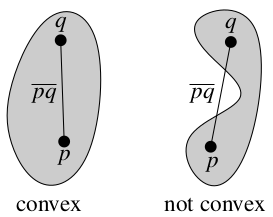
\includegraphics[width=0.5\linewidth]{images/convexhull1.png}
                \caption{}
                \label{fig:convexhull1}
            \end{subfigure} &
            \begin{subfigure}{.5\textwidth}
                \centering
                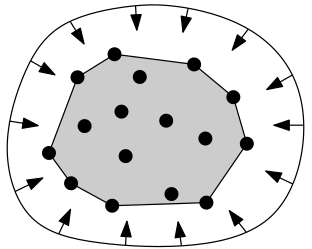
\includegraphics[width=0.5\linewidth]{images/convexhull2.png}
                \caption{}
                \label{fig:convexhull2}
            \end{subfigure}
        \end{tabular}
        \caption{Example of Convexity}
    \end{figure}

    \begin{itemize}
        \item The computation of \textbf{planar convex hull} was one of the first computational geomtry problems. 
        \item \emph{Convexity 1}: A subset $S$ of the plane is \textbf{convex} if and only if for any pair of points $p, q \in S$, the line segment $\overline{pq}$ is completely contained in $S$. See Fig. \ref{fig:convexhull1}. The \emph{convex hull}, $\mathcal{CH}(S)$, of a set $S$ is the smallest convex set that contains $S$; it is the intersection of all convex sets that contain $S$. 
        \item \emph{Convexity 2}: How to compute the convex hull of a finite set $P$ of $n$ points in the plane? The area enclosed in the shaded region is the convex hull of $P$. See Fig. \ref{fig:convexhull2}. It is the unique convex polygon whose vertices are points from $P$.
    \end{itemize}


    \begin{figure}[h]
        \centering
        \begin{tabular}{cc}
            \begin{subfigure}{.5\textwidth}
                \centering
                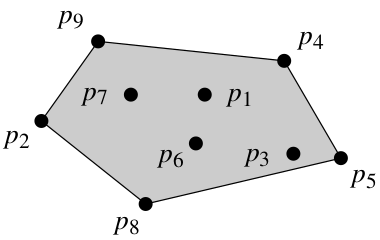
\includegraphics[width=0.5\linewidth]{images/convexhull3.png}
                \caption{}
                \label{fig:convexhull3}
            \end{subfigure} &
            \begin{subfigure}{.5\textwidth}
                \centering
                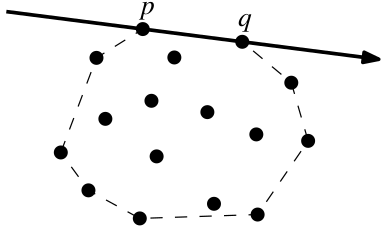
\includegraphics[width=0.5\linewidth]{images/convexhull4.png}
                \caption{}
                \label{fig:convexhull4}
            \end{subfigure}
        \end{tabular}
        \caption{computing convex hull}
    \end{figure}


    \begin{itemize}
        \item Fig. \ref{fig:convexhull3}: To compute a convex hull of a set of points, $P = \{p_1, p_2, ... p_9\}$, we compute a list of those vertices from $P$ that are the vertices of $\mathcal{CH}(P)$, i.e. $\{p_4, p_5, p_8, p_2, p_9\}$, and list them in clockwise order. Defining $\mathcal{CH}(P)$ as a convex polygon is more useful than discussing the intersection of all convex sets. 
        \item Fig. \ref{fig:convexhull4}: For points $p$ and $q$ that are endpoints of an edge and that are in $P$, we direct a line through $p$ and $q$, and if $\mathcal{CH}(P)$ lies to one side, then all points in $P$ must lie to that side of the $\overline{pq}$ line. And if all points of $P \setminus \{p, q\}$ lie to one side of $\overline{pq}$, then $\overline{pq}$ is an edge of the $\mathcal{CH}(P)$.
    \end{itemize}
    %%%%%%%%%

    %%%
    \subsection{\textbf{Algorithm} \textsc{SlowConvexHull}($P$) - Naive $O(n^3)$}
        \emph{Input}: A set $P$ of points in a plane.

        \emph{Output}: A list $\mathcal{L}$ cotnaining vertices of $\mathcal{CH}(P)$ in clockwise order. 

        \begin{enumerate}
            \item $E \leftarrow \emptyset$
            \item $\forall$ ordered pairs $(p, q) \in P \times P$, where $p \neq q$
            \item \hspace{0.5cm} \textbf{do} \emph{valid} $\leftarrow$ \textbf{true}
            \item \hspace{1cm} $\forall r \in P, r \neq p, r \neq q$
            \item \hspace{2cm} \textbf{do} \textbf{if} $r$ lies to the left of directed line from $p$ to $q$
            \item \hspace{3cm} \textbf{then} \emph{valid} $\leftarrow$ \textbf{false}
            \item \hspace{1cm} \textbf{if} \emph{valid} \textbf{then} Add add directed edge $\overrightarrow{pq}$ to $E$.
            \item From the set $E$ of edges, construct a list $\mathcal{L}$ of vertices of $\mathcal{CH}(P)$, sorted in clockwise order. 
        \end{enumerate}

        \begin{itemize}
            \item \emph{*Assume for now that methods to test if a point is to the right or left of a line is available. Assume this primative operation is O(1).}
            \item \emph{*initially ignores the degenerate case, where a point r may lie on $\overrightarrow{pq}$}. To consider the degeneracy, must specify that $\overrightarrow{pq}$ is an edge of $\mathcal{CH}(P)$ if and only if all other $r \in P$ lie strictly on the right or left of $\overrightarrow{pq}$, or they lie on the open line segment $\overline{pq}$.
            \item \emph{Problems with rounding error could arise should coordinates are represented in floating point numbers, leading to unexpected results.}
            \item Constructing $\mathcal{L}$ takes about $O(n^2)$ time. For an edge $e_1 \in E$, take the source and destination points, add them to $\mathcal{L}$. Using the destination point of $e_1$, find the $e_2$ that has that as it's origin, and add $e_2$'s destination point to $\mathcal{L}$. Repeat until only one edge is left in $E$. 
            \item Complexity Analysis: 
                \begin{itemize}
                    \item Check each of the $n^2 - n$ \emph{pairs} of points. For each pair, look at $n - 2$ other points to see if they lie to one side. Total: $O(n^3)$.
                    \item Constructing $\mathcal{L}$ is $O(n^2)$.
                    \item Total overall: $O(n^3)$.
                \end{itemize}
        \end{itemize}
        %%%%%%%%%

        %%%
        \subsection{\textbf{Algorithm} ConvexHull($P$) - Incremental Algorithm $O(n \log n)$}

        Needs only a sorting method and a method to test if three points can make a right turn. 

        Briefly: Given the set $P$ of points on a plane, sort the points $p_1, ..., p_n$ ordering them by their x-coordinate. Compute the convex hull vertices on the \emph{upper hull} first, from left to right, from point $p_1$ to $p_n$. Then copute the convex hull vertices of the \emph{lower hull} from right to left, from $p_n$ to $p_1$. 

        Updating of the upper hull after adding point $p_i$ is important. Suppose there is a list $\mathcal{L}_{up}$ containing the left to right upper hull vertices seen thus far, $\{p_1, ..., p_{i - 1}\}$. Append $p_i$ to $\mathcal{L}_{up}$. It is correct if $p_i$ is the rightmost point so far, and if the last three points in $\mathcal{L}_{up}$ make a \emph{right} turn. Move on to $p_{i+1}$ if $p_i$ can be in the upper hull thus far. If a left turn is made, delete the middle point from the upper hull, and keep rechecking the last three points until a right turn is verified.

        \begin{figure}[h]
            \centering
            \begin{tabular}{cc}
                \begin{subfigure}{.5\textwidth}
                    \centering
                    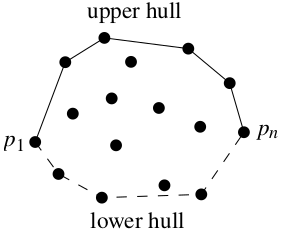
\includegraphics[width=0.5\linewidth]{images/chalgo1.png}
                    \caption{}
                    \label{fig:chalgo1}
                \end{subfigure} &
                \begin{subfigure}{.5\textwidth}
                    \centering
                    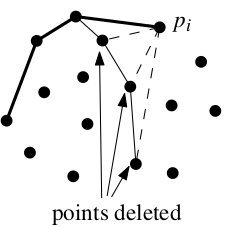
\includegraphics[width=0.5\linewidth]{images/chalgo2.png}
                    \caption{}
                    \label{fig:chalgo2}
                \end{subfigure}
            \end{tabular}
            \caption{Convex Hull Algorithm}
        \end{figure}


        \emph{Input}: A set $P$ of points in a plane.

        \emph{Output}: A list $\mathcal{L}$ cotnaining vertices of $\mathcal{CH}(P)$ in clockwise order. 

        \begin{enumerate}
            \item Sort the points by x-coordinate, resulting in sequence $p_1, ..., p_n$.
            \item Put $p_1$ and $p_2$ in $\mathcal{L}_{up}$, with $p_1$ as the first point. 
            \item \textbf{for} $i \leftarrow 3$ \textbf{to} $n$
            \item \hspace{1cm} \textbf{do} Append $p_i$ to $\mathcal{L}_{up}$
            \item \hspace{2cm} \textbf{while} $| \mathcal{L}_{up} | > 2$ \textbf{and} the last three points in $\mathcal{L}_{up}$ don't make a right turn, 
            \item \hspace{2.5cm} \textbf{do} delete the middle of the last three points in $\mathcal{L}_{up}$
            

            \item Put points $p_{n}$ and $p_{n - 1}$ in $\mathcal{L}_{low}$, with $p_n$ as the first point. 
            \item \textbf{for} $i \leftarrow n - 2$ \textbf{down to} 1
            \item \hspace{1cm} \textbf{do} Append $p_i$ to $\mathcal{L}_{low}$
            \item \hspace{2cm} \textbf{while} $| \mathcal{L}_{low} | > 2$ \textbf{and} the last three points in $\mathcal{L}_{low}$ don't make a right turn, 
            \item \hspace{2.5cm} \textbf{do} delete the middle of the last three points in $\mathcal{L}_{low}$
            
            \item Remove the first and last points from $\mathcal{L}_{low}$ (avoid duplicate points of where upper and lower hull meet).
            \item Append $\mathcal{L}_{low}$ to $\mathcal{L}_{up}$, call the result $\mathcal{L}$
            \item \textbf{return} $\mathcal{L}$
        \end{enumerate}

        \begin{itemize}
            \item We assumed no two points have the same x-coordinate. To consider that, sort same-x-coord points by their y-coord.
            \item We will say for three collinear points (make a straight line), they make a left turn.
            \item Points very close together could create sharp left turns. For these, consider them the same point by rounding.
            \item Algorithm will compute a closed polygonal chain. 
            \item \textbf{Theorem} \emph{The convex hull of a set of n points in the plane can be computed in $O(n \log n)$ time}.
            \item \textbf{Proof}: See \cite{berg08} page 8. 
                \begin{itemize}
                    \item Correctness of computation of upper hull (and lower) is proof by induction. Briefly, the set $\mathcal{L}_{up}$ of $\{p_1, p_2\}$ is trivially the upper hull. $\mathcal{L}_{up}$ containing the chain $\{p_1, ..., p_{i - 1}\}$ is known, by induction to only make right turns, and that all points fall below the chain. When considering point $p_i$, be know that $p_1$ is the smallest point and $p_i$ will be the biggest point thus far. There can be no points above the old chain, because if there were, then it would have to lie between $p_{i-1}$ and $p_i$ in sorted order. 
                    \item Sorting the points can be done in $O(n \log n)$ time. Computing upper hull is done in $O(n)$ time, because the for loop is executed a linear number of times, as any extra executions (from the while loop) is bound by $n$ since extra points can only be deleted onces during the hull construction. Similarly, lower hull construction is $O(n)$ time. Therefore total time for computing convex hull is $O(n \log n)$. 
                \end{itemize}
        \end{itemize}


        \begin{figure}[h]
            \centering
            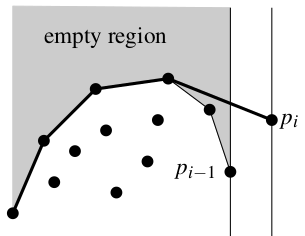
\includegraphics[width=0.3\linewidth]{images/chalgo3.png}
            \caption{Convex Hull Algorithm - Correctness}
            \label{fig:chalgo3}
        \end{figure}


        %%%%%%%%%
        

        

        


    %%%
    \subsection{3D Convex Hull}
    \label{subsec:3dconvexhull}
    Introduced (background) in \cite{berg08} CH. 11
    %%%%%%%%%

    \pagebreak
    % END %%%%%%%%%%%%%%%%%%%%%%%%%%%%%%%%%%%%%%%%%%%%%%%%%%%%%%%%%%%%%%%%%%%%


    \section{Hello World}
    \label{sec:hello} % section label
                      % to link sections within file, 
                      % do \hyperref[label]{text}
        Link to \hyperref[sec:figures]{Figures section}

\cbcolor{dkgreen}
\cbstart
\begin{lstlisting}
(; This is a comment. ;)

(; This is a 
   multi-lined comment. ;)
\end{lstlisting}
\cbend


        \subsection{Fonts and Styles:}
            \begin{itemize}
                \item hello world
                \item \lstinline!world world!
                \item \sf{hello world}
                \item \textsc{Hello World}
                \item $\Theta(n)$
            \end{itemize}

        \subsection{Enum List Style:}
            \begin{enumerate}[label=(\alph*)]
                \item One
                \item Two
                \item Three
            \end{enumerate}

        \subsection{A basic Table:}
            \begin{center}
                \begin{tabular}{||cc||}
                    \hline
                    hello & world \\
                    \hline
                \end{tabular}
            \end{center}

        \subsection{Figure}
        \label{sec:figures}
            Basic single figure (commented out):
            % \begin{figure}[h]
            %     \centering
            %     \includegraphics[width=0.7\linewidth]{FILE_PATH}
            %     % \caption{}
            %     \label{fig:FILE_NAME}
            % \end{figure}

            Code environment:
\begin{lstlisting}[stepnumber=0]
int main() {
    cout << "Hello World" << endl;
}
\end{lstlisting}

            One way to put code side-by-side:

\begin{tabular}{l|l}
\hline
\begin{minipage}[h]{0.5\textwidth}
    \begin{lstlisting}[stepnumber=0]
    <animal.h>= // C++
    class Animal {
    ...
    };
    \end{lstlisting}
\end{minipage}
&                  % remember  '&' between cells in a row
\begin{minipage}[h]{0.5\textwidth}
    \begin{lstlisting}[stepnumber=0]
    <animal.cpp>= // C++
    ...
    \end{lstlisting}
\end{minipage} \\ % remember '\\' at the end of each row
\hline
\end{tabular}

                One way to align multiple (2) figures in a row:
                % \begin{figure}[h]
                %     \centering
                %     \begin{tabular}{cc}
                %         \begin{subfigure}{.5\textwidth}
                %             \centering
                %             \includegraphics[width=1\textwidth]{FILE_PATH1}
                %             \label{fig:FILE_NAME1}
                %         \end{subfigure} &
                %         \begin{subfigure}{.5\textwidth}
                %             \centering
                %             \includegraphics[width=1\textwidth]{FILE_PATH2}
                %             \label{fig:FILE_NAME2}
                %         \end{subfigure}
                %     \end{tabular}
                %     \label{fig:MULTI_NAME}
                % \end{figure}

    %%%%%%%%%%%%%%%%%%%%%%%%%%%%%%%%%%%%%%%%%%%%%%%%%%%%%%%%%%%%%%%%%%%%%
    \begin{thebibliography}{1}
        \bibitem[1]{berg08}Mark de Berg, Otfried Cheong, Marc van Kreveld, and Mark Overmars. 2008. Computational Geometry: Algorithms and Applications (3rd ed. ed.). Springer-Verlag TELOS, Santa Clara, CA, USA.
        \bibitem[2]{key2}Hi
    \end{thebibliography}
    % END %%%%%%%%%%%%%%%%%%%%%%%%%%%%%%%%%%%%%%%%%%%%%%%%%%%%%%%%%%%%%%%%%%%%

\end{document}